%%%%%%%%%%%%%%%%%%%%%%%%%%%%%%%%%%%%%%%%%%%%%%%%%%%%%%%%%%%%%%%%%%%%%%%%
%                                                                      %
%     File: Thesis_Results.tex                                         %
%     Tex Master: Thesis.tex                                           %
%                                                                      %
%     Author: Andre C. Marta                                           %
%     Last modified :  2 Jul 2015                                      %
%                                                                      %
%%%%%%%%%%%%%%%%%%%%%%%%%%%%%%%%%%%%%%%%%%%%%%%%%%%%%%%%%%%%%%%%%%%%%%%%

\chapter{Investing in a new product when the firm is already active}
\label{chapter:2}



%%%%%%%%%%%%%%%%%%%%%%%%%%%%%%%%%%%%%%%%%%%%%%%%%%%%%%%%%%%%%%%%%%%%%%%%
\section{Introduction}
\label{section:2_intro}

We consider now the case in which a firm that is already active, with an established product in the market, and has the opportunity to invest in a new and more profitable product, replacing the old one.

By an established product we mean that it is so well recognized in the market that its unitary price is not influenced by the demand level, assuming a fixed price, given by
%, even before we decide to invest, the firm already produces a certain product. We also consider that the product is \textit{stable} in the market, in the sense that it's a recognized product, resulting in a demand function that is not influenced by the demand level. Instead it's given by
\begin{equation}
p_0=1-\alpha K_0
\label{p0}
\end{equation}
where $\alpha$ stands for a capacity sensibility parameter and $K_0$ for the capacity of production of this product, that we will call the old product.

However, the same does not hold for the new product. When the innovation breakthrough takes place, the firm has the option to invest and immediately start to produce the new product. Since this one is a new product, susceptible to the consumers' demand, its unitary price function is considered to be the same as stated in Section \ref{section:overview}, that is,
\begin{equation}
p_1(X_t)=(\theta-\alpha K_1)X_t
\label{p1}
\end{equation}
where $\theta$ stands for the innovation level after the breakthrough, $\alpha$ for the same sensitivity parameter as in the old product, $K_1$ for the capacity of production of the new product and $X_t$ for the demand level at time $t$.

The instantaneous profit function with respect to each product is given by $\pi_i, \ i \in \{0,1\}$, and it is obtained by multiplying the unitary price function by the production capacity. %, that is, $\pi_i(X_t)=p_i(X_t) K_i$. 


%\vspace{4mm}
%\begin{figure}[!htb]
%	\centering
%	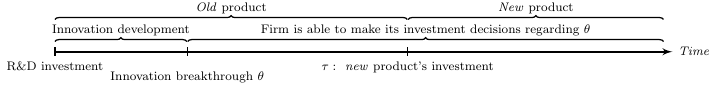
\includegraphics[width=\textwidth]{Prob2_CapOpt/2_timelinet.PNG}
%	\caption{Timeline representing the two possible different stages of production and associated decisions. Time is set to start at the innovation breakthrough.}
%	\label{2_time}
%\end{figure}

\begin{figure}
	\centering
	
	\begin{tikzpicture}[y=1cm, x=1cm, thick, font=\footnotesize]    
	\usetikzlibrary{arrows,decorations.pathreplacing}
	
	
	
	% time line week
	\draw[line width=1.2pt, ->, >=latex'](0,0) -- coordinate (x axis) (14,0) node[right] {\textit{Time}}; 
	\foreach \x in {0,3,9}
	\draw (\x cm,3pt) -- (\x cm,-3pt);
	%\foreach \x in {current time,  , $\tau$, 3} \draw (\x,0.1) -- (\x,-0.1) node[below] {\x};
	\draw (0,0) node[below=3pt] (a) {$\text{R\&D investment}$} node[above=3pt] {};
	\draw (3,0) node[below=9pt] (a) {$\text{Innovation breakthrough $\theta$}$} node[above=3pt] {};
	\draw (9,0) node[below=3pt] (a) {$\text{$\tau$ new product's investment}$} node[above=3pt] {};
	
	brace
	\node (start_p) at (0,0.6) {};
	\node (end_p) at (8.99,0.6) {};
	\draw [brace_top] (start_p.north) -- node [above, pos=0.5] {$\text{\textit{Old product}}$} (end_p.north);
	
	%brace
	\node (start_pn) at (9.01,0.6) {};
	\node (end_pn) at (13.8,0.6) {};
	\draw [brace_top] (start_pn.north) -- node [above, pos=0.5] {$\text{\textit{New product}}$} (end_pn.north);
	
	%brace
	%\node (start_pn) at (12.01,0.6) {};
	%\node (end_pn) at (13.8,0.6) {};
	%\draw [brace_top] (start_pn.north) -- node [above, pos=0.5] {$\text{new product}$} (end_pn.north);
	
	
	% top brace
	\node (start_t) at (0,0.1) {};
	\node (end_t) at (2.99,0.1) {};
	\draw [brace_top] (start_t.north) -- node [above, pos=0.5] {$\text{Innovation development}$} (end_t.north);
	
	% top brace
	\node (start_week) at (3.01,0.1) {};
	\node (end_week) at (13.8,0.1) {};
	\draw [brace_top] (start_week.north) -- node [above, pos=0.5] {$\text{Firm is able to make its investment decisions regarding $\theta$}$} (end_week.north);
	
	\end{tikzpicture}
	\caption{Timeline representing the two possible different stages of production and associated decisions. Time is set to start at the innovation breakthrough.}
	\label{2_time}
\end{figure}



Since the firm is not interested to invest before the innovation process reaches level $\theta$, it is not relevant, for the investment decision, to consider what happened before. Therefore the initial time is set to start at the instant the breakthrough takes place. %($t_\theta$).  
Hence the optimal investment time will occur $\tau^*$ time units after the breakthrough, as presented on Figure \ref{2_time}.

Recall that at the moment we decide to invest, we need to pay $\delta K_1$ related to sunk costs. We assume also that upon investment in the new product, the old product is no longer in the market.
%, that the established product is in that precise instant retired from the market and that the investment is an irreversible decision.



As in the previous section, two models will be derived. The first one is the benchmark model, which accounts for the model as explained in the introduction. The second one is the capacity optimization model, which considers the maximized the long-run profit by choosing the optimal capacity $K_1$ to invest on. Comparative statics w.r.t. both models will be presented afterwards.
%consists takes into account the maximized instantaneous profit in function of the production capacity related with the new product $K_1$. Comparative statics of both models will be made afterwards.

%Here, as in Problem 1, we consider a unique possibly jump in the innovation process $\{ \theta_t, t \geq 0 \}$, that is denoted by $\theta$. 


%%%%%%%%%%%%%%%%%%%%%%%%%%%%%%%%%%%%%%%%%%%%%%%%%%%%%%%%%%%%%%%%%%%%%%%%
\section{Stopping Problem}
\label{section:2_theory}



\subsection{Benchmark Model}
\label{subsec:2_bm}

We want to find when is the best time to invest in the new product, knowing that the firm produces an established product, that it's not influenced by the demand level and which profit function is given by 
\begin{equation}
\pi_0=(1-\alpha K_0)K_0,
\label{pi0}
\end{equation}
and when the replacement happens, the firm will be immediately and solely produce a product which profit function corresponds to
\begin{equation}
\pi_1(X_t) =(\theta-\alpha K_1)K_1 X_t.
\label{pi1}
\end{equation}

Assuming that the investment decision must be made in finite time, our optimal stopping problem may be written as
\begin{equation}
\sup _\tau \mathds{E}^{X_0=x} \left[  \int_0^\tau \pi_0e^{-rs} ds +  \left( \int_\tau^\infty \pi_1(X_s)e^{-rs}ds -e^{-r\tau}\delta K_1 \right) \mathds{1}_{\{ \tau < \infty \}} \right].
\label{eq:prob2}
\end{equation}

The first integral corresponds to the discounted profit associated to the old product from the time when the innovation level $\theta$ is reached (considered here to be its initial instant) until the time when the firm decides to invest in the new product (denoted by $\tau$). The second integral corresponds to the long term discounted profit associated to the new product, obtained after investing. Subtracting to it discounted sunk costs $e^{r \tau} \delta K_1$, we obtain the cash-flow associated to the investment decision.

We can simplify this problem in order to have a standard optimal stopping problem with null running cost function.
Starting by conditioning \eqref{eq:prob2} to the time when the investment should happen and using Tower rule it follows that \eqref{eq:prob2} is equal to
\begin{equation}
\sup _\tau \mathds{E}^{X_0=x} \left[ \mathds{E}^{\tau} \left[  \int_0^\tau \pi_0e^{-rs} ds +  \left(  \int_\tau^\infty \pi_1(X_s)e^{-rs}ds -e^{-r\tau} \delta K_1   \right) \mathds{1}_{\{ \tau < \infty \}} \right] \right].
\label{eq:prob21}
\end{equation}
Since expectation is a linear operator, we can simplify each of the integrals separately.

Note that in the leftmost integral of \eqref{eq:prob21}, as previously written, the instantaneous profit associated to the old product does not depend on the demand level and all the parameters are deterministic. Then we easily solve the integral, simplifying its expression as
\begin{align}
\mathds{E}^{\tau} \left[\int_0^\tau \pi_0e^{-rs} ds \right] 
&= \mathds{E}^{\tau} \left[ \int_0^\tau p_0K_0e^{-rs} ds \right] \nonumber \\
&= \mathds{E}^{\tau} \left[ \int_0^\tau (1-\alpha K_0) K_0e^{-rs} ds \right] \nonumber \\
&= \mathds{E}^{\tau} \left[ (1-\alpha K_0) K_0 \frac{1-e^{-r \tau}}{r} \right] \nonumber\\
&= \mathds{E}^{\tau} \left[ \frac{\pi_0}{r} (1-e^{-r \tau}) \right]
\label{g2}
\end{align}

Following a similar approach as in Section \ref{subsec:1_bm}, when deducing \eqnref{prob1:h}, and assuming that $\tau$ is finite with probability 1, the leftmost expected value of the rightmost integral can also be simplified as
\begin{align}
\mathds{E}^{\tau} \left[  \int_\tau^\infty \pi_1(X_s)e^{-rs} ds -e^{-rt}\delta K_1 \right]
&\underset{v:=s-\tau}{=}  \mathds{E}^{\tau} \left[  e^{-rt} \left( \int_0^\infty p_1(X_{v+t}) K_1e^{-rv} dv -\delta K_1 \right) \right] \nonumber \\
& \quad = \mathds{E}^{\tau} \left[ e^{-rt} \left( \int_0^\infty (\theta-\alpha K_1)X_{v+t} K_1e^{-rv} dv -\delta K_1 \right) \right] \nonumber \\
& \quad = \mathds{E}^{\tau} \left[ e^{-rt} \left( \int_0^\infty (\theta-\alpha K_1)X_{v+t} K_1e^{-rv} dv -\delta K_1 \right) \right] \nonumber \\
& \quad = e^{-r\tau} \left( \frac{(\theta-\alpha K_1)K_1 X_\tau}{r-\mu} -\delta K_1 \right)
\label{h2}
\end{align}
where $X_\tau$ is taken to be the demand level at the time when the new product starts being produced. Recall, from the previous section, that expression \eqref{h2} only holds if the assumptions of Fubini's Theorem hold, which particularly implies that $r-\mu>0$.

Let's denote $F$ as the value function solution to \eqref{eq:prob21}. Plugging expressions \eqref{g2} and \eqref{h2} in \eqref{eq:prob21}, getting rid of the expectation conditional to time when the investment decision is made and using (again) the Tower rule, we obtain that, assuming the investment decision to be made in finite time, $F$ may be written as
\begin{equation}
F(x)=\frac{\pi_0}{r}+ \sup _\tau \mathds{E}^{X_0=x} \left[ e^{-r\tau}\left(\frac{(\theta-\alpha K_1)K_1 X_\tau}{r-\mu} - \left( \delta K_1  +\frac{\pi_0}{r}\right)  \right) \right],
\label{prob235}
\end{equation}
%which corresponds to the sum of a constant term with a standard optimal stopping problem with null running cost function, as we wanted. This is the effect of dealing with a very stable product, which doesn't depend on the current demand level, allowing us to simply this much its expression.
and therefore this problem can be analysed as in Chapter \ref{chapter:1}, corresponding to the case of a constant term plus an optimal stopping problem with null running cost function. 
%Note that the terminal cost function here, given by $h(x)=\frac{(\theta-\alpha K_1)x}{r-\mu} - \left( \delta K_1  +\frac{\pi_0}{r}\right)$, is a non-decreasing function in $x$ of the type $h(x,\underline{\psi})=k(\underline{\psi})x-j(\underline{\psi})$ with $k(\underline{\psi})$ and $j(\underline{\psi}) > 0$ functions, $\underline{\psi}$  a vector corresponding to the deterministic arguments and $x$ corresponding to the stochastic argument.

Considering $V$ to be the optimal stopping problem present in \eqref{prob235}, that is
\begin{equation}
V(x)=  \sup _\tau \mathds{E}^{X_0=x} \left[ e^{-r\tau}h(X_\tau) \right] 
=\sup _\tau \mathds{E}^{X_0=x} \left[ e^{-r\tau}\left(\frac{(\theta-\alpha K_1)K_1 X_\tau}{r-\mu} - \left( \delta K_1  +\frac{\pi_0}{r}\right)  \right) \mathds{1}_{ \{\tau < \infty \} }\right].
\end{equation} 

Following all the steps presented before, we propose as candidate for the continuation region $\mathcal{C}=\{x \in \mathds{R}: x<x_B^* \}$, with $x^*_B$ being the demand level that triggers the investment. Since $V$ satisfies the HJB variational inequality \eqref{HJB} it takes the form of
%$V$ is such that it must verify the HJB variational inequality \eqref{HJB} regarding values on the continuation and stopping region. As was written in Section \ref{bc_ro}, it follows that $V$ is such that
\begin{equation}
V(x)=\begin{cases} a_2 x^{d_1} &\ , \ x \in \mathcal{C} \\
\frac{(\theta-\alpha K_1)K_1 x}{r-\mu} - \left( \delta K_1  +\frac{\pi_0}{r}\right) &\ , \ x \in \mathcal{S}
\end{cases}.
\end{equation}

The coefficient $a_2$ and the threshold value $x_B^*$ are found by value matching \eqref{valuematch} and smooth pasting \eqref{smoothpasting} conditions, expressed by the corresponding system
\begin{equation}
\begin{cases} a_2(x_B^*)^{d_1}=\frac{(\theta-\alpha K_1)K_1 x_B^*}{r-\mu} - \left( \delta K_1  +\frac{\pi_0}{r}\right) \\
a_2d_1(x_B^*)^{d_1-1}=\frac{(\theta-\alpha K_1)K_1}{r-\mu}
\end{cases},
\label{eq:sistema2}
\end{equation}
leading to
\begin{align}
&x_B^*=\frac{d_1}{d_1-1} \frac{ \delta K_1  +\frac{\pi_0}{r} }{\theta-\alpha K_1} \frac{r-\mu}{K_1} \label{2_xB} \\
&a_2=\left( \delta K_1 +\frac{\pi_0}{r}\right) \frac{(x_B^*)^{-d_1}}{d_1-1} \label{2_aB}
\end{align}


Plugging the results stated above on the expression of $F$ \eqref{prob235}, it leads to
\begin{equation}
F(x)=\frac{\pi_0}{r}+\begin{cases} a_2 x^{d_1} &\ , \ x<x^*_B \\
\frac{(\theta-\alpha K_1)K_1 x}{r-\mu} - \left( \delta K_1  +\frac{\pi_0}{r}\right) &\ , \ x\geq x_B^*
\label{2:Fbm}
\end{cases}
\end{equation}
with an associated optimal stopping time defined as in \eqref{stoptime}.




\subsection{Capacity Optimization Model}
\label{subsec:2_com}

As considered in Chapter \ref{chapter:1}, we now extend the previous model, by allowing the firm to optimally choose the capacity of the new product.
This optimal stopping problem can be stated as
\begin{align}
F^*(x)&=\sup _\tau \mathds{E}^{X_0=x} \left[ \max_{K_1} \left\{ \int_0^\tau \pi_0e^{-rs} ds + e^{-r\tau} \left( \int_\tau^\infty \pi_1(X_s)e^{-rs}ds -\delta K_1 \right) \mathds{1}_{ \{\tau < \infty \} } \right\} \right] \nonumber \\
&= \frac{\pi_0}{r}+ \sup _\tau \mathds{E}^{X_0=x} \left[ e^{-r\tau} \max_{K_1}   \left\{ \frac{(\theta-\alpha K_1)K_1X_\tau}{r-\mu} - \left( \delta K_1  +\frac{\pi_0}{r}\right)   \right\} \mathds{1}_{ \{\tau < \infty \} } \right],
\label{eq:o2}
\end{align}
where the expression is simplified in a similar way as done in the previous section, and using the fact that $\pi_0$ is deterministic.

Denoting the non-maximized terminal function by $h$ with the dependence on the capacity parameter $K_1$ highlighted, we have that
\begin{equation}
h(x,K_1)= \frac{(\theta-\alpha K_1)K_1 x}{r-\mu} - \left( \delta K_1  +\frac{\pi_0}{r}\right).
\label{2_h}
\end{equation}
%$h$ is a second order polynomial with respect to the capacity, meaning that it exists an optimal capacity level $K_1^*$ that maximizes it.

Note that $h$ is a second order polynomial with respect to the capacity and its expression corresponds to the terminal function in the previous chapter minus a constant term ($\frac{\pi_0}{r}$). Thus, by studying the first and second derivatives of $h$, we obtain the same results as achieved in Section \ref{subsec:1_com}: its first and second partial derivatives are, respectively, given by \eqref{1_dK} and \eqref{1_d2K}. Therefore the maximizer of $h$ in \eqref{2_h} is the same in \eqref{eq:K41}, that is,
\begin{equation}
K^*_1:=\text{arg} \max_{K_1} h(x,K_1) = \frac{\theta}{2\alpha}-\frac{\delta (r-\mu)}{2 \alpha x}, \ \forall x.
\label{eq:Kopt2}
\end{equation}

Evaluating $h$ at its optimal capacity level and denoting by $h^*$, we obtain that its expression is given by
\begin{equation}
h(x,K^*)=\frac{\pi_0}{r} + \frac{(\theta x -\delta (r-\mu))^2}{4 \alpha (r-\mu) x}
,
\label{2_h*} 
\end{equation}
from which follows that our problem, as described in \eqref{eq:o2}, can be stated as
\begin{equation}
F^*(x)=\frac{\pi_0}{r}+ \sup _\tau \mathds{E}^{X_0=x} \left[ e^{-r\tau}   \left( \frac{\pi_0}{r} + \frac{(\theta X_\tau -\delta (r-\mu))^2}{4 \alpha (r-\mu) X_\tau} \right) \mathds{1}_{ \{\tau < \infty \} } \right],
\label{eq:opt22}
\end{equation}
which consists in a standard stopping optimal problem with null running cost function plus a positive constant term.

%We will focus now on the optimal stopping problem and denote it by $V^*$, that is,

Denoting $V^*$ as the value function associated to the optimal stopping problem in \eqref{eq:opt22}, the optimization problem can be stated as
\begin{equation}
V^*(x)=\sup _\tau \mathds{E}^{X_0=x} \left[ e^{-r\tau}   \left( \frac{\pi_0}{r} + \frac{(\theta X_\tau -\delta (r-\mu))^2}{4 \alpha (r-\mu) X_\tau} \right) \mathds{1}_{ \{\tau < \infty \} } \right]
\label{2_V*}
\end{equation}
which is again a standard optimal stopping problem with null running cost function. Therefore, invoking results presented on Chapter \ref{chapter:bc}, it follows that $V^*$ is such that
\begin{equation}
V^*(x)=\begin{cases} b x^{d_1}  \ , \ x \in \mathcal{C} \\
\frac{\pi_0}{r}+ \frac{(\theta x -\delta (r-\mu))^2}{4 \alpha (r-\mu) x} \ , \ x \in \mathcal{S}
\end{cases}.
\label{2_V*3}
\end{equation}
%with $d_1$ being the positive root of the polynomial described in \eqref{d1}.

Considering that the continuation region should be of the form $\mathcal{C}= \{ x \in \mathds{R}: x< x^*_C \}$ - stating that the firm should postpone the investment for small demand values, in particular, smaller than $x_C^*$ -, $b$ and $x_C^*$ are found by value matching \eqref{valuematch} and smooth pasting \eqref{smoothpasting} conditions, hereunder expressed
\begin{equation}
\begin{cases} b (x_C^*)^{d_1}=\frac{\pi_0}{r} + \frac{(\theta x_C^* -\delta (r-\mu))^2}{4 \alpha (r-\mu) x_C^*}\\
b d_1(x_C^*)^{d_1-1}=\frac{\theta^2 (x_C^*)^2 -\delta^2 (r-\mu)^2}{4 \alpha (r-\mu) (x_C^*)^2}
\end{cases}
.
\label{eq:2_sistema}
\end{equation}

We obtain two possible positive roots for the threshold level:
\begin{align*}
x^*_{C,1}&=\frac{r-\mu}{(d_1-1) \theta ^2 r}
\left(
d_1 \left(2 \alpha pi_0 + \delta  \theta  r \right) +
\sqrt{(\delta  \theta  r)^2 + 4 d_1^2 \alpha \pi_0 \left( \alpha \pi_0 +\delta  \theta  r \right)} \right)\\
x^*_{C,2}&=\frac{r-\mu}{(d_1-1) \theta ^2 r}
\left(
d_1 \left(2 \alpha \pi_0 + \delta  \theta  r \right) -
\sqrt{(\delta  \theta  r)^2 + 4 d_1^2 \alpha \pi_0 \left( \alpha \pi_0 +\delta  \theta  r \right)} \right).
\end{align*}
However, since the coefficient $b$ associated to it takes a negative value, we exclude $x^*_{C,2}$. As explained in the previous chapter, considering such $b$ would be an absurd. Consequently, we obtain that the threshold level and coefficient $b$ in \eqref{eq:2_sistema} are, respectively, given by
\begin{align}
&x_C^*=\frac{r-\mu}{(d_1-1) \theta ^2 r}
\left(
d_1 \left(2 \alpha \pi_0 + \delta  \theta  r \right) +
\sqrt{(\delta  \theta  r)^2 + 4 d_1^2 \alpha \pi_0 \left( \alpha \pi_0 +\delta  \theta  r \right)} \right) \label{eq:prob2_xC}\\
&b=\left( \frac{K_0 (\alpha  K_0-1)}{r}+\frac{(\theta  x^*_C-\delta  (r-\mu ))^2}{4 \alpha  x^*_C (r-\mu )} \right)(x_C^*)^{-d_1}. \nonumber
\end{align}

Plugging the results above on \eqref{eq:opt22} it follows that $F^*$ corresponds to
\begin{equation}
F^*(x)=\frac{\pi_0}{r}+\begin{cases} b x^{d_1}  &\ , \ x < x_C^* \\
\frac{\pi_0}{r}+ \frac{(\theta x -\delta (r-\mu))^2}{4 \alpha (r-\mu) x} &\ , \ x \geq  x_C^*
\end{cases},
\label{2_V*2}
\end{equation}
leading to an optimal stopping time as defined in \eqref{stoptime}.


Following a similar approach as in Section \ref{subsec:1_com}, we evaluate $K^*_1$ at the threshold demand level $x_C^*$, obtaining
\begin{equation}
K^*_C=\frac{\theta }{2 \alpha }-\frac{\delta  (d_1-1) \theta ^2 r}{2 \alpha  \left(\sqrt{4 \alpha  d_1^2 \pi_0 (\alpha  \pi_0+\delta  \theta  r)+\delta ^2 \theta ^2 r^2}+d_1 (2 \alpha  \pi_0+\delta  \theta  r)\right)}.
\label{3_K*}
\end{equation}

%Denoting $X_0$ as the demand value at the innovation breakthrough, we have that $K^*_C$ represents the optimal capacity to invest on the new product, considering that the initial demand is smaller than the value that triggers the investment (i.e. $X_0 \leq x^*_C$). However it does not correspond to the optimal capacity to invest if $X_0$ is greater than $x_C^*$. In this case, it is given by evaluating $K^*_1$ at $X_0$.
%Such quantity represents the optimal capacity to invest on the new product at the first instant, after the innovation breakthrough, the demand process reaches $x_C^*$. It does not correspond to the best one if, at the instant the innovation breakthrough happens, there is a demand level greater than $x^*_C$. In this case the optimal capacity to invest is given by evaluating $K^*_1$ at $X_0$ (the demand value at the innovation breakthrough such that $X_0>x_C^*$).











%%%%%%%%%%%%%%%%%%%%%%%%%%%%%%%%%%%%%%%%%%%%%%%%%%%%%%%%%%%%%%

\section{Comparative Statics}

In this section we analyse the results obtained regarding $x^*_B$, $x^*_C$ and $K^*_C$. As we have considered in Chapter 3, we compare $x^*_B$ and $x^*_C$.
% the threshold obtained in the benchmark model and then the one obtained on the capacity optimization model as well as the associated optimal capacity to invest. Comparisons between both thresholds and the optimal capacity are made in the end of the chapter.

\subsection{Benchmark Model}
\label{2_bm}
%In this section we study the behaviour of the decision threshold $x^*_B$ and $x^*_{C}$ and $K^*$ as described in \eqref{ass3}, with the different parameters.


\begin{prop}
	\label{2_prop1}
The decision threshold $x^*_B$ increases with $ \delta$, decreases with $\theta$ and does not have a monotonic behaviour with $K_0, \ K_1, \ r$. Regarding the sensibility parameter $\alpha$, $x_B^*$ increases with it when $\theta < \frac{K_1}{ K_0^2} (K_0+K_1 r \delta)$, and decreases otherwise. Regarding volatility $\sigma$,  $x_B^*$ increases with it when $d_1 \in (1,\frac{1}{2} (3+\sqrt{5}))$ and decreases when $d_1 \in \left(\frac{1}{2} (3+\sqrt{5}), \infty \right)$.
\end{prop}

\textbf{Proof:}

Regarding the formula obtained for  $x^*_B$ \eqref{2_xB}, we immediately conclude that the decision threshold increases with $\delta$ and decreases with $\theta$.


Regarding $K_0$, we conclude that
\begin{align*}
\frac{\partial x^*_B ( K_0 ) }{\partial K_0}= 
\frac{d_1 (r-\mu )}{r (d_1-1)K_1(\theta-\alpha K_1)} (1-2\alpha K_0)
=
\begin{cases}
>0 &\ \text{for} \ K_0<\frac{1}{2 \alpha}\\
<0 &\ \text{for} \ K_0>\frac{1}{2 \alpha}
\end{cases},
\end{align*}
since the expression represented in fraction is always positive.


Regarding $K_1$, we obtain that
\begin{align*}
\frac{\partial x^*_B ( K_1 ) }{\partial K_1}= 
\frac{d_1 (r-\mu )}{ (d_1-1)K_1(\theta-\alpha K_1)}  \left( \frac{\alpha (\frac{\pi_0}{r}+K_1 \delta )}{\theta-\alpha K_1} -\frac{ \frac{\pi_0}{r}+K_1 \delta }{K_1}+ \delta \right).
\end{align*}


The first term in the equation is always positive. Thus we only need to evaluate the second term (between brackets). Manipulating it and taking into account that the capacity level cannot be negative
\footnote{We obtain that 
	$$\frac{\alpha (\frac{\pi_0}{r}+K_1 \delta )}{\theta-\alpha K_1} -\frac{ \frac{\pi_0}{r}+K_1 \delta }{K_1}+ \delta =
\frac{d_1 (r-\mu) (2K_1 \pi_0 \alpha+K^2_1r \alpha \delta -\pi_0 \theta)}{(d_1-1)K_1^2r(\theta-\alpha K_1)^2}$$
which roots are given by
$$ 2K_1 \pi_0 \alpha+K^2_1r \alpha \delta -\pi_0 \theta =0  \ \Leftrightarrow \ K_1=\frac{-\pi_0 \pm \sqrt{\alpha \pi_0 (\pi_0 + r \delta \theta)}}{ r\alpha \delta}.
$$
Since the capacity chosen $K_1$ must be positive, we obtain a single root, $K_1=\frac{-\pi_0 + \sqrt{\alpha \pi_0 (\pi_0 + r \delta \theta)}}{ r\alpha \delta}$, that leads to the result presented.}
, it follows that
\begin{align*}
\frac{\partial x^*_B ( K_1 ) }{\partial K_1}= 
\begin{cases}
>0 &\ \text{for} \ K_1>\frac{-\pi_0+\sqrt{\alpha \pi_0 (\pi_0 + r \delta \theta)}}{ r\alpha \delta}\\
<0 &\ \text{for} \ K_1 \in \left[ 0, \frac{-\pi_0+\sqrt{\alpha \pi_0(\pi_0 + r \delta \theta)}}{ r\alpha \delta} \right]
\end{cases},
\end{align*}
from which we obtain that $x^*_B$ does not have a monotonic behaviour with $K_1$.


Regarding parameter $\alpha$, we obtain that

\begin{align*}
\frac{\partial x^*_B ( \alpha ) }{\partial \alpha}= 
\frac{d_1 (r-\mu )}{ (d_1-1)(\theta-\alpha K_1)}  \left( \frac{\frac{K_0(1-\alpha K_0)}{r}+ \delta K_1  }{\theta-\alpha K_1} -\frac{ K_0^2}{r K_1} \right).
\end{align*}
Again, the first term is positive. Simplifying the second term
\footnote{Reducing to the same denominator it follows that the rightmost expression corresponds to
	$$\frac{\frac{\pi_0}{r}+ \delta K_1  }{\theta-\alpha K_1} -\frac{ K_0^2}{r K_1} =
	\frac{r K_1 \frac{K_0(1-\alpha K_0)}{r}+ \delta K_1  -K_0^2(\theta-\alpha K_1)}{r K_1(\theta-\alpha K_1)},$$
	which is equal to zero when
	$$  K_1 K_0(1-\alpha K_0)+ r\delta K_1^2  -K_0^2(\theta-\alpha K_1)= K_0K_1+r\delta K_1^2-K_0^2 \theta=0 \ \Rightarrow \ \theta=\frac{K_0 K_1 +K_1^2 r\delta}{K_0^2}.
	$$
	},
it follows that
\begin{align*}
\frac{\partial x^*_B ( \alpha ) }{\partial \alpha}= 
\begin{cases}
>0 &\ \text{for} \ \theta < \frac{K_0 K_1 +K_1^2 r\delta}{K_0^2}\\
<0 &\ \text{for} \ \theta > \frac{K_0 K_1 +K_1^2 r\delta}{K_0^2}.
\end{cases}
\end{align*}

Note that the sign of the partial derivative does not depend on $\alpha$, but instead on both capacity levels $K_0$ and $K_1$, discount rate $r$ and sensibility parameter $\delta$.


Regarding $\sigma$, we conclude that
$$    \frac{\partial x^*_B ( \sigma ) }{\partial \sigma}= 
\underbrace{ \frac{(r-\mu )  \left(\delta  K_1+\frac{\pi_0}{r}\right)}{(d_1-1) K_1 (\theta -\alpha  K_1)}}_{(1)}
\underbrace{ \left(\frac{2 \mu }{\sigma ^3}+\frac{\frac{4 \mu  \left(\frac{1}{2}-\frac{\mu }{\sigma ^2}\right)}{\sigma ^3}-\frac{4 r}{\sigma ^3}}{2 \sqrt{\left(\frac{1}{2}-\frac{\mu }{\sigma ^2}\right)^2+\frac{2 r}{\sigma ^2}}}\right) }_{(2)}
\underbrace{ \left( 1- \frac{d_1}{(d_1-1)^2} \right) }_{(3)} =
\begin{cases}
>0 \ \text{for} \ d_1 \in \left(1,\frac{1}{2} (3+\sqrt{5}) \right]\\
<0 \ \text{for} \ d_1 \in \left(\frac{1}{2} (3+\sqrt{5}), \infty \right)
\end{cases}.$$
Forthwith, we agree that expression (1) is positive.
%Taking into account our initial assumptions about $r, \ \mu$ and profits associated to the old and the new product, it follows that the leftmost expression is always positive.
Manipulating expression (2), we obtain that
\begin{align}
\frac{2 \mu }{\sigma ^3}+\frac{\frac{4 \mu  \left(\frac{1}{2}-\frac{\mu }{\sigma ^2}\right)}{\sigma ^3}-\frac{4 r}{\sigma ^3}}{2 \sqrt{\left(\frac{1}{2}-\frac{\mu }{\sigma ^2}\right)^2+\frac{2 r}{\sigma ^2}}}<0  &\Leftrightarrow  \mu d_1-r<0 \nonumber \\
&\Leftrightarrow \frac{\mu}{2}-\frac{\mu^2}{\sigma^2}+\mu \sqrt{\left( \frac{1}{2}-\frac{\mu}{\sigma^2}\right)^2+\frac{2r}{\sigma^2}}-r<0 \nonumber \\
%&\Leftrightarrow \frac{1}{4}-\frac{r^2}{\mu^2}+\frac{2r}{\sigma^2}<\frac{r^2}{\mu^2}-\frac{r}{\mu} \nonumber \\
&\Leftrightarrow \frac{r}{\mu}\left(1-\frac{r}{\mu} \right) <0 \label{mud1-r},
\end{align}
which holds true as $r>\mu$. %for the two possible cases: when $\mu<0$ and $\mu>0$.
Analysing expression (3), we have that the polynomial $d_1^2-d_1-1$ has roots on $\left\{\frac{1}{2} (3-\sqrt{5}),\frac{1}{2} (3+\sqrt{5}) \right\}$. Since $d_1>1$, the first root is not admissible. Consequently, we obtain that expression (3) is negative for $d_1 \in \left(1,\frac{1}{2} (3+\sqrt{5}) \right]$, and positive for $d_1 \in \left(\frac{1}{2} (3+\sqrt{5}), \infty \right)$.



Regarding parameter $r$ we obtained complex derivatives, from which we weren't able to derive any analytical result. However, as it will be shown later, numerical results show that $x_B^*$ behaves in a non-monotonic way with $r$.
%However, as it will be showed right after this proof, using Mathematica we obtained that $x^*_B$ behaves in a non-monotonic way with it.

Regarding $\mu$, as the sign of the derivatives is not either clearly positive or negative, we could not assess analytically if $x^*_B$ has a monotonic behaviour w.r.t. $\mu$. But as we will present later, numerical illustrations suggest that $x_B^*$ decreases with $\mu$.
\begin{flushright}
	$\square$
\end{flushright}

%We weren't able to deduce any analytical result regarding the drift value $\mu$. However, after many numerical experiments, we observed that $x_B^*$ decreases with $\mu$, as it's showed on Figure \ref{fig:2_x3}.

%Similarly, we were not able to study analytically the behaviour of $x_B^*$ with $\mu$. But, as we will present later, numerical experiments suggest that $x_B^*$ decreases with $\mu$.

\subsection{Capacity Optimization Model}
\label{2_com}


\begin{prop}
	\label{2_prop2}
The decision threshold $x^*_C$ increases with $\delta$, decreases asymptotically with $\theta$ and has a non-monotonic behaviour with $\mu, \ r, \  \alpha$ and $K_0$.
\end{prop}

\textbf{Proof:}

For the sake of simplicity, in this proof, we consider $\phi$ as in \eqref{phi}, which is always positive and well-defined, and we define
$\psi:=4 d_1^2 \alpha \pi_0  (\delta  \theta  r+\alpha \pi_0 )+\delta ^2 \theta ^2 r^2$, which is also positive.
% and well-defined w.r.t to our assumptions.
%Recall also that $\pi_0>0$ stands for the profit function associated to the new product.

Regarding $\delta$, we immediately conclude that

\begin{align*}
\frac{\partial x^*_C ( \delta ) }{\partial \delta}= \frac{(r-\mu ) \left(\frac{4 d_1^2 \theta  r \pi_0 +2 \delta  \theta ^2 r^2}{2 \sqrt{\psi }}+d_1 \theta  r\right)}{(d_1-1) \theta ^2 r}>0.
\end{align*}

Regarding $\theta$, we obtain that
\begin{align*}
	\frac{\partial x^*_C ( \theta) }{\partial \theta}= \frac{ \theta (r-\mu ) \left(\frac{4 \delta  d_1^2 r \alpha \pi_0 +2 \delta ^2 \theta  r^2}{2 \sqrt{\psi }}+\delta  d_1 r\right)- 2 (r-\mu ) \left(d_1 (\delta  \theta  r+2 \alpha \pi_0 )+\sqrt{\psi }\right)}{(d_1-1) \theta ^3 r}.
\end{align*}
Although we weren't able to evaluate the sign of preceding expression due its the complexity, we analyse its asymptotic behaviour. This is possible since we assume no upper limit for innovation levels  $\theta$.

%The denominator is positive since $d_1>1$.
%Manipulating the numerator, we obtain that it has
%it simplifies to
%$$ (r-\mu) \frac{\delta ^2 \theta ^2 r^2+\delta  d_1 \theta  r \left(2 d_1 \alpha \pi_0 -\sqrt{\psi }\right)-2 \left(2 d_1 \sqrt{\psi } \alpha \pi_0 +\psi \right)}{\sqrt{\psi} }=,$$
%two roots associated ($\theta \in \{ -\frac{4 d_1^2 \alpha \pi_0 }{\delta  r}, 0 \}$)
%\footnote{
%	In order to calculate the roots of the numerator we have
%	$$ (r-\mu) \frac{\delta ^2 \theta ^2 r^2+\delta  d_1 \theta  r \left(2 d_1 \alpha \pi_0 -\sqrt{\psi }\right)-2 \left(2 d_1 \sqrt{\psi } \alpha \pi_0 +\psi \right)}{\sqrt{\psi} }=0$$
%	 $$\Rightarrow \ 2 \alpha  \delta  d_1^2 \theta  \pi_0 r- d_1 \sqrt{\psi } (4 \alpha  \pi_0+\delta  \theta  r)+\delta ^2 \theta ^2 r^2-2 \psi = -d_1 (4 \alpha  \pi_0+\delta  \theta  r) \sqrt{4 \alpha  d_1^2 \pi_0 (\alpha  \pi_0+\delta  \theta  r)+\delta ^2 \theta ^2 r^2}-2 \alpha  d_1^2 \pi_0 (4 \alpha  \pi_0+3 \delta  \theta  r)-\delta ^2 \theta ^2 r^2=0 $$
%}, which are impossible given the domain of the problem.
%Thus, since by evaluating for a certain $\theta>0$, we obtain $\frac{\partial x^*_B ( \theta) }{\partial \theta}<0$, the result holds.


%Since we assume that innovation levels have no upper limit, we evaluated them asymptotically.
Denoting $\theta_A:=\frac{(r-\mu )}{(d_1-1) r}  \left(\sqrt{\delta ^2 r^2}+\frac{\delta  r \left(\sigma ^2 (\phi +1)-2 \mu \right)}{2 \sigma ^2}\right)>0$ we obtain that $x^*_C$ asymptotically decreases in order of $\frac{\theta_A}{\theta}$, that is,  

$$x^*_C(\theta) \sim \frac{\theta_A}{\theta} \ \Leftrightarrow \ \lim_{\theta \to \infty} \frac{x^*_C(\theta)}{\frac{\theta_A}{\theta}}=1.$$

%Regarding parameters $\mu, \ r, \ \alpha$ and $K_0$ we obtained complex derivatives, from which we weren't able to derive any analytical result. However as it will be shown later, numerical results suggest that $x_C^*$ behaves in a non-monotonic way with each of them.
Regarding parameters $\mu, \ r, \ \alpha$ and $K_0$ we obtained complex derivatives, from which we weren't able to derive any analytical result. However, as it will be shown later, numerical results show that $x_C^*$ behaves in a non-monotonic way with each of them.

\begin{flushright}
	$\square$
\end{flushright}


%Although we couldn't obtain any analytical (strong) evidence, after different experiments done using \textit{Mathematica} and its function \texttt{Manipulate}, we obtained that decision thresholds $x^*_B$ and $x^*_C$ increase with volatility $\sigma$. An example is showed on Figure \ref{fig:2_x2}.







\subsubsection{Numerical comparisons between the Benchmark and the Capacity Optimization Models}

In a similar way as done in Chapter \ref{chapter:1}, using software \textit{Mathematica}, we perform numerical simulations to illustrate the above results. 
In addition to the values considered in the previous chapter, we also assume $K_0=50$ (and $K_1=100$).

%We start by illustrating how does $x^*_B$ and $x^*_C$ are related by the capacity level $K$, on which $x^*_B$ is dependent. One can see on Figure \ref{fig:Kvar} that conclusions mentioned on the proof (including that $x^*_B(0)=x^*_C$) hold.


\begin{figure}[!htb]
	\begin{subfigmatrix}{2}
		\subfigure[$\delta \in (0,1)$]{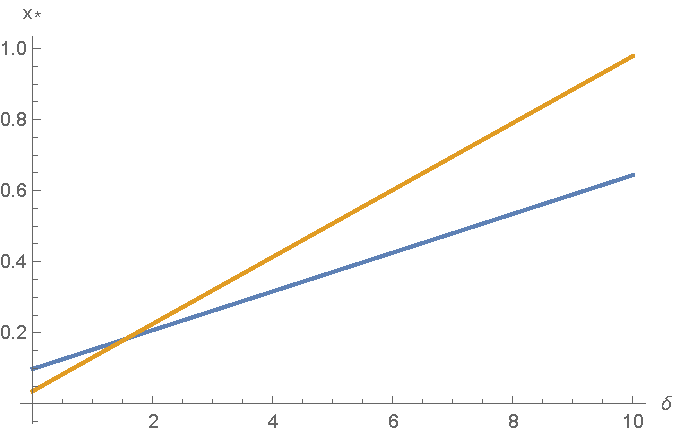
\includegraphics[width=0.45\textwidth]{Prob2_CapOpt/xopt_delta.pdf}}
		\subfigure[$\sigma \in (0,1)$]{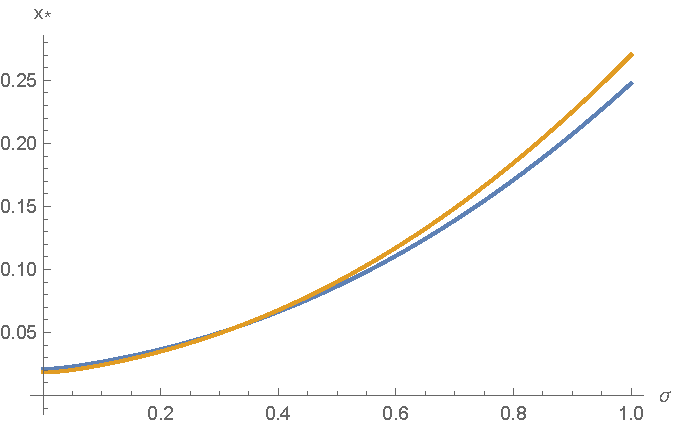
\includegraphics[width=0.45\textwidth]{Prob2_CapOpt/xopt_sigma.pdf}}
	\end{subfigmatrix}
	\caption{Behaviour of the threshold value with respect to the benchmark model (blue) and the capacity optimized model (orange) and parameters with which $x^*_B$ increases $\delta$ (a) and $\sigma$ (b).}
	\label{fig:2_x2}
\end{figure}


Figures \ref{fig:2_x2} (a) and (b) show the behaviour of both thresholds by changing $\delta$ and $\sigma$, respectively. 
%They are on line with the theoretical results (Propositions \ref{2_prop1} and \ref{2_prop2}).
%On Figure \ref{fig:2_x2}, we obtained similar results to the ones on Section 2. Both threshold values increase with sensibility parameter $\delta$ and volatility $\sigma$. 
The first result is motivated by the fact that a higher $\delta$ reflects a larger investment (sunk) cost, which is only incurred if there is a demand level large enough such that the investment is worthwhile.

The second one is justified by the growing uncertainty (of the demand). Although we were not able to derive analytically this result regarding the threshold $x_C^*$, it is widely common that a larger volatility postpones the investment decision \cite{dixit:book}. 
%Since it has a high variance, the demand has a great amplitude of values, which delays the investment decision, only made when the demand reaches a high level. This is in accordance to what is described in \cite{dixit:book}.


\begin{figure}[!htb]
	\begin{subfigmatrix}{2}
		\subfigure[$\theta \in (1,10)$]{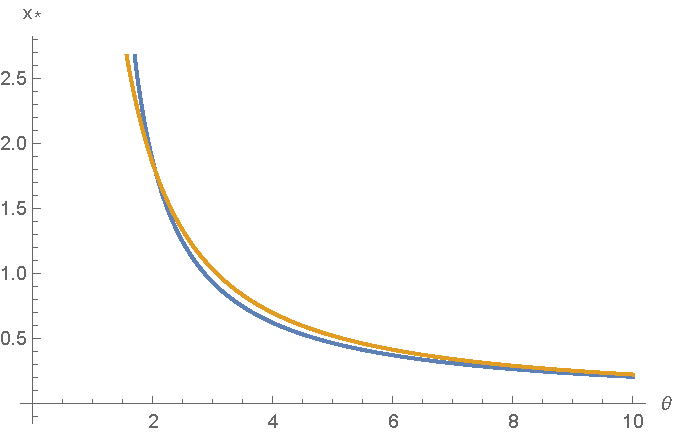
\includegraphics[width=0.45\textwidth]{Prob2_CapOpt/xopt_theta.pdf}}
		\subfigure[$\mu \in ( -r,r )$ ]{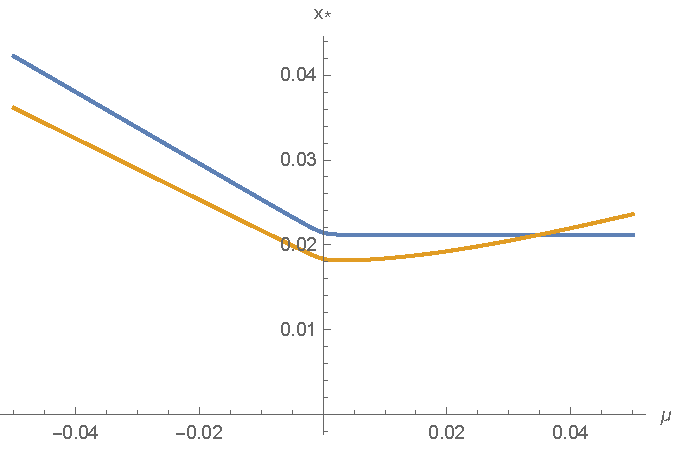
\includegraphics[width=0.45\textwidth]{Prob2_CapOpt/xopt_mu.pdf}}
	\end{subfigmatrix}
	\caption{Behaviour of the threshold value with respect to the benchmark model (blue) and the capacity optimized model (orange) and parameter with which  $x^*_B$ decreases $\theta$ (a) and $\mu$ (b).}
	\label{fig:2_x3}
\end{figure}



On Figure \ref{fig:2_x3} (a) we observe that, similarly to what was described on Chapter 3, both threshold levels decrease with innovation level, meaning that the firm is eager to invest when the technology improvement is more significant.

Regarding expectations about the market evolution (illustrated in Figure \ref{fig:2_x3} (b)), we see that in a declining market ($\mu<0$) both thresholds decrease approximately in a linear rate. However the same is not verified on a growing market ($\mu>0$). The threshold associated to the Benchmark Model still decreases, but in a weaker rate than in a declining market, whereas $x^*_C$ increases with $\mu$. Again, we believe this happens in view of the invested capacity associated to each threshold (as, with increasing $\mu$, the optimal capacity $K^*_C$ also increases, and therefore the firm tends to invest later).

% Although the threshold level associated to the Benchmark Model decreases with $\mu$ in what seems to be a linear way for negative values of $\mu$ and almost negligible for positive values of $\mu$, the same doesn't happen to the threshold level associated to the capacity optimization model. This last one, seems to increase for positive values of $\mu$. 

%The same happened considering other values for parameters $K_0, \ \alpha, \ \delta, \ \theta$. Regarding $\sigma$, we obtained that when increasing the volatility, the value of $\mu$ associated with the stationary point happens for values of $\mu$ greater than 0.

\begin{figure}[!htb]
	\begin{subfigmatrix}{3}
		\subfigure[$r \in (\mu,1)$, $\mu=0.01$ and $\sigma=0.9$]{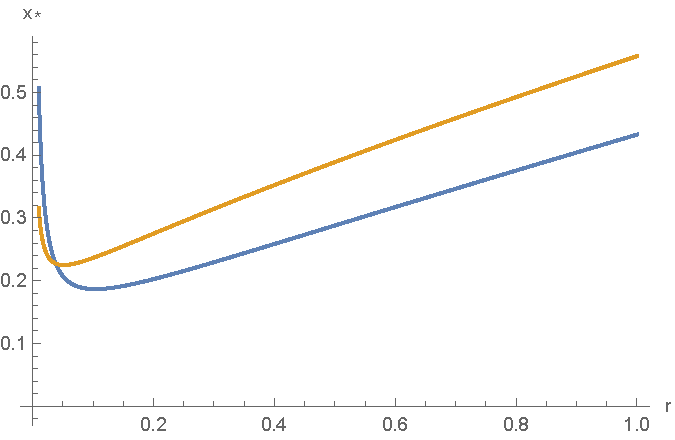
\includegraphics[width=0.32\textwidth]{Prob2_CapOpt/xopt_r.pdf}}
		\subfigure[$K_0 \in ( 0, \frac{1}{\alpha}=100 )$ ]{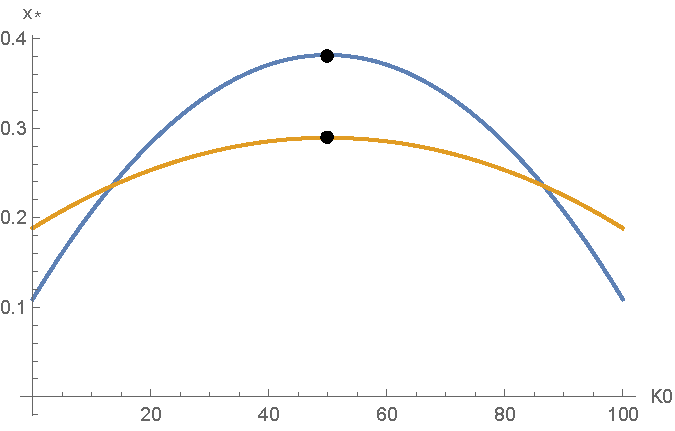
\includegraphics[width=0.32\textwidth]{Prob2_CapOpt/xopt_k0.pdf}}
		\subfigure[$K_1 \in (0, \frac{\theta}{\alpha}=1000 )$]{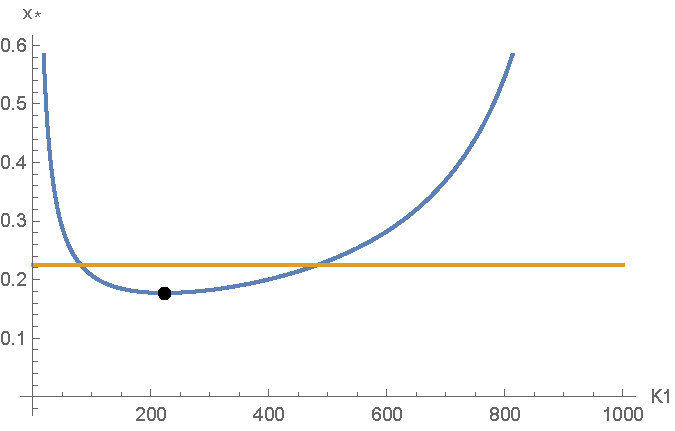
\includegraphics[width=0.32\textwidth]{Prob2_CapOpt/xopt_k1.pdf}}
	\end{subfigmatrix}
	\caption{Behaviour of the threshold value with respect to the benchmark model (blue) and the capacity optimized model (orange) and parameters with which $x^*_B$ has a non-monotonic behaviour $r$ (a), $K_0$ (b) and $K_1 (c)$.}
	\label{fig:2_x1}
\end{figure}

%On Figure \ref{fig:2_x1} we have that a non-monotonic behaviour was also observed on parameters $r$, $K_0$ and $K_1$, being this last one only valid for the Benchmark Model.
%On Figure \ref{fig:2_x1}, we observe that both threshold level behave in a non-monotonic way with $r$ and $K_0$.

On Figure \ref{fig:2_x1} (a) we observe that, concerning each model, exists a discount rate that leads to a minimal demand threshold and that it is associated to small values of $r$. Unfortunately, we were not able to derive its analytical expression.
% thethe leftmost plot we can see that a minimum demand threshold is observed for small values of discount rate $r$. Unfortunately we couldn't derive its analytical expression.

Interestingly, as seen on Figure \ref{fig:2_x1} (b), 
%regarding the capacity of old product,
a maximum demand threshold is observed on both models when the capacity level $K_0$ is exactly equal to $\frac{1}{2 \alpha}$ (which, on this case, takes the value $K_0=50$). This quantity is motivated by the profit function associated to the established product, in the sense that a capacity of $\frac{1}{2 \alpha}$ leads to the maximization of $\pi_0$. Therefore, for $K_0$ assuming quite smaller or larger values than $\frac{1}{2 \alpha}$, the firm obtains a relative low profit in the old product and, consequently, the idea of investing in a new product gets more attractive to the firm, which is reflected by the small threshold levels.
%This values comes from the expression $\alpha K_0 \pi_0=\alpha K_0 (1-\alpha K_0)$ included on both expressions of $x_B^*$ \eqref{2_xB} and $x^*_C$ \eqref{eq:prob2_xC}.


Regarding the capacity associated to the new product, we notice on Figure \ref{fig:2_x1} (c), that (as expected) it only affects $x_B^*$. We observe that a large $x_B^*$ is associated to either quite small or quite large values of $K_1$. The first one is explained by the fact that, to invest in a small quantity, the demand needs to be large enough such that the expected long-run $\pi_1$ (and investment costs) overcome the profit associated to the established product. The second one supports that the larger the capacity to invest on, the larger the expected $\pi_1$ is as well as associated investment costs. Hence, a larger value of demand is needed, in order to justify the investment made. A minimum triggering value is observed at $K_1=\frac{-\pi_0+\sqrt{\alpha \pi_0(\alpha \pi_0+\delta \theta r)}}{r\alpha \delta}$ (which, on this case, takes the value $K_1\simeq  223$).

%Regarding parameter $K_1$, its value doesn't affect threshold $x^*_C$, since it takes into account the optimal capacity $K^*_C$. However, when it comes to the threshold $x^*_B$ we have that it achieves a minimum value at $K_1=\frac{\pi_0+\sqrt{\alpha \pi_0(\pi_0+\delta \theta r)}}{r\alpha \delta}$, as it's represented on the bottom plot. Note that the standard value considered was $K_1=100$ and that it's associated a threshold $x_B^*$ smaller than the threshold $x_C^*$. This is one of the reasons why the demand threshold $x_B^*$ appears to be smaller than $x_C^*$ in most cases. However as showed in Figure \ref{fig:Kvar} (b), we have that the value function $F^*$ (associated to the threshold $x_C^*$) will always be greater than the value function $F$ (associated to the threshold $x_B^*$).
	
	\begin{figure}[!htb]
		\begin{subfigmatrix}{2}
			\subfigure[$\alpha \in (0,1)$ and $\theta=10>\frac{K_1}{ K_0^2} (K_0+K_1 r \delta)$]{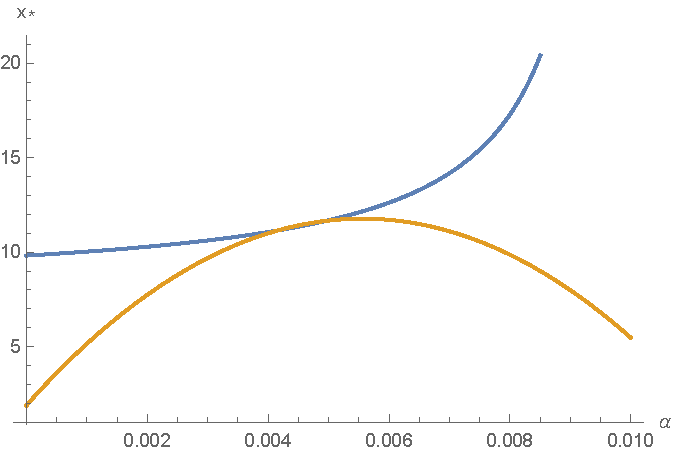
\includegraphics[width=0.45\textwidth]{Prob2_CapOpt/xopt_alpha_O.pdf}}
			\subfigure[$\alpha \in (0,1) $ and $\theta=1<\frac{K_1}{ K_0^2} (K_0+K_1 r \delta)$]{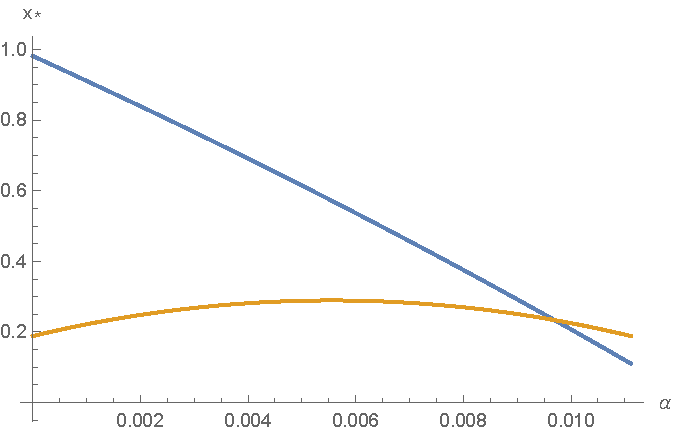
\includegraphics[width=0.45\textwidth]{Prob2_CapOpt/xopt_alpha_op.pdf}}
		\end{subfigmatrix}
		\caption{Behaviour of the threshold value with respect to the benchmark model (blue) and the capacity optimized model (orange) and sensibility parameter $\alpha$.}
		\label{fig:2_x4}
	\end{figure}
	
Figure \ref{fig:2_x4} highlights the two possible behaviours of $x^*_B$ regarding parameter $\alpha$. As stated in Proposition \ref{2_prop1}, we observe that for values of $\theta$ greater than $\frac{K_1}{ K_0^2} (K_0+K_1 r \delta)$ (which, in this case, is approximately 1.235), $x^*_B$ decreases with $\alpha$ (as represented on (a)). For greater values than that quantity, $x^*_B$ increases (as represented on (b)). We propose that this unexpected behaviour happens due to the influence of both $\pi_0$ and $\pi_1$.
% In this case, $\frac{K_1}{ K_0^2} (K_0+K_1 r \delta)$ is approximately 1.235.
Although we were not able to derive any analytical result concerning $x^*_C$, we conclude that it behaves non-monotonically with $\theta$, confirming the stated on Proposition \ref{2_prop2}.


% it's represented the behaviour of $x^*_B$ with $\alpha$, as written on Proposition \label{3_prop2}. Considering the fixed values considered before, we obtain a $\theta$-threshold equal to $\frac{K_1}{ K_0^2} (K_0+K_1 r \delta)=1.23457$. One can see on Figure \ref{fig:2_x4} when that testing for innovation levels greater (leftmost) and smaller (rightmost) than the mentioned threshold, we verify what was deduced: that $x^*_B$ behaves in either an increasing or decreasing way with $\alpha$ for certain levels of innovation, while $x_C^*$ always behave in a non-monotonic way.
	%Note that on most of the plots you have that the threshold $x_C^*$ has an associated capacity level ($K^*(x_C^*)$) greater than the one considered ($K_1=100$), resulting in values $x^*_B$ smaller than $x_C^*$, contrarily to what happened on the previous section.

\subsection{Optimal Capacity Level}

In this section we analyse the optimal capacity level $K^*_C$, whose formula is provided in \eqref{3_K*}. Due to its complex expression, we are just able to deduce analytical results concerning the asymptotic behaviour of $K^*_C$ with $\theta$. However, the numerical results obtained lead us to conclude that it has a similar behaviour to the optimal capacity presented on Chapter \ref{chapter:1}, whose formula corresponds to equation \eqref{prob1:K*}.
%Now we analyse optimal capacity level $K^*_C$, that is given by evaluating $K^*$ on demand level $x^*_C$ and as it is written in \eqref{3_K*}.

\begin{prop}
Asymptotically, the optimal capacity level $K^*_C$ grows in a linear rate with $\theta$. Also, $K^*_C$ has a non-monotonic behaviour with $K_0$. 
\end{prop}

\textbf{Proof:}

Regarding innovation level $\theta$, assuming that it has no upper limit, it's possible to evaluate its behaviour asymptotically. Denoting $\theta_K:=\frac{\sigma ^2 \left(\sqrt{\delta ^2 r^2}+\delta  r\right)}{\alpha  \left(2 \sigma ^2 \sqrt{\delta ^2 r^2}+\delta  r \left(\sigma ^2 (\phi +1)-2 \mu \right)\right)}>0$, we obtain that $K^*_C$ increases on order of $\theta_K \theta$, that is,
$$K^*_C(\theta) \sim \theta_K \theta \ \Leftrightarrow \ \lim_{\theta \to \infty}  \frac{K^*_C}{\theta_K \theta}=1 $$


The non monotonic behaviour of $K^*_C$ with $K_0$ is illustrated in Figure \ref{fig:2_k0}.
\begin{flushright}
	$\square$
\end{flushright}
\vspace{2cm}
%Although it wasn't possible to derive any (strong) analytical solution about te behaviour of the other parameters, numerically we obtain robust results. By manipulating each parameter, using command \texttt{Manipulate}, we obtained no different behaviours from the ones showed hereunder.

%The results obtained regarding parameters $\mu, \ \sigma,\ r, \ \alpha$ and $\theta$  were similar to the ones obtain for the optimal capacity level on the previous section.  Since $K^*_C$ depends on value $x_C^*$, it is expected to observe similiar behaviours regarding the studied parameters. 


\begin{figure}[!htb]
	\centering
	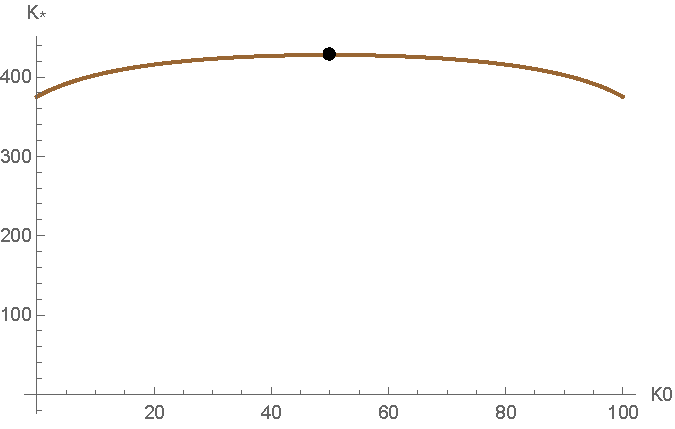
\includegraphics[width=0.45\textwidth]{Prob2_CapOpt/koptx_k0.pdf}
	\caption{Behaviour of the optimal capacity regarding the threshold value $x^*_C$ considering capacity levels $K_0 \in [0, 100)$ and its highest values at $\frac{1}{2 \alpha}=50$ (black).}
	\label{fig:2_k0}
\end{figure}

%Starting with the capacity level of the old product $K_0$, 
Figure \ref{fig:2_k0} shows that the highest optimal capacity level $K^*_C$ happens for $K_0=\frac{1}{2 \alpha}$.
We note that this stresses previous observations: if the firm is committed to a larger investment, then it impacts the investing timing, postponing it.
% This is motivated by the results obtained for $x^*_C$, as seen on Figure \ref{fig:2_x1}, which also reaches its highest value at $\frac{1}{2 \alpha}$.

\vspace{0.5cm}

\begin{figure}[!htb]
	\begin{subfigmatrix}{3}
		\subfigure[$\mu \in ( -r,r )$ ]{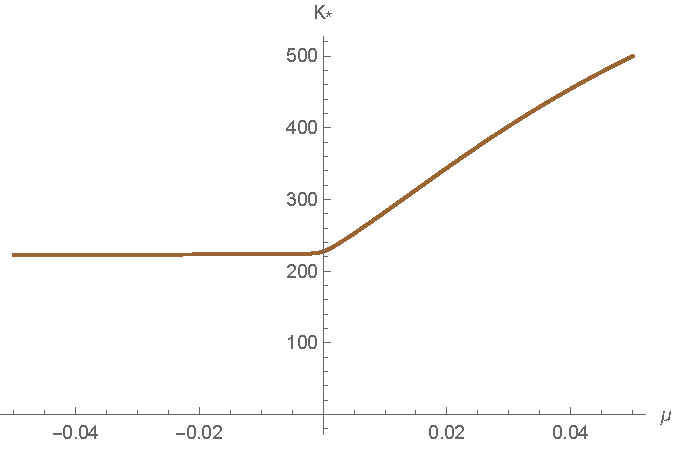
\includegraphics[width=0.32\textwidth]{Prob2_CapOpt/koptx_mu.pdf}}
		\subfigure[$\sigma \in (0,1)$]{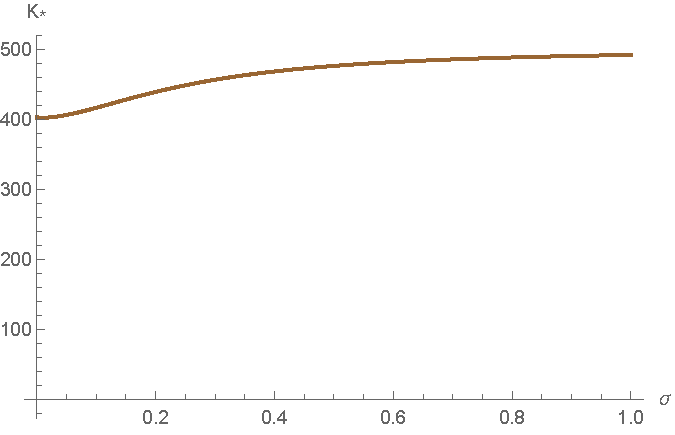
\includegraphics[width=0.32\textwidth]{Prob2_CapOpt/koptx_sigma.pdf}}
		\subfigure[$ \theta \in ( 1, 10 )$]{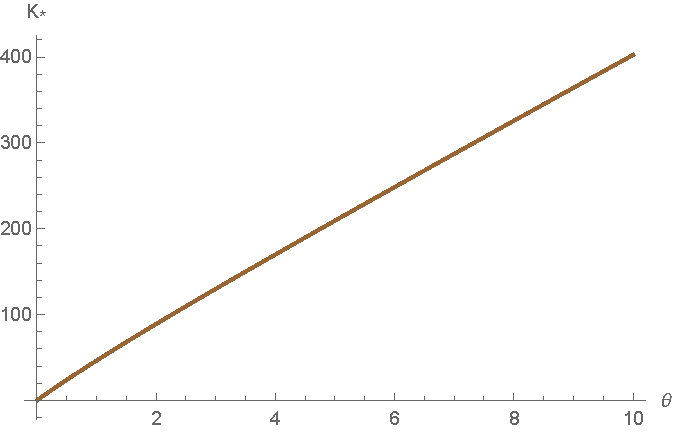
\includegraphics[width=0.32\textwidth]{Prob2_CapOpt/koptx_theta.pdf}}
	\end{subfigmatrix}
	\caption{Behaviour of the optimal capacity regarding the threshold value $x^*_C$ and increasing parameters $\mu$ (a), $\sigma$ (b) and $\theta$ (c).}
	\label{fig:2_k1}
\end{figure}

Figure \ref{fig:2_k1} illustrates that $K^*_C$ increases with both drift, volatility and innovation level, as it happened in the previous section. 
Note, on Figure \ref{fig:2_k1} (a), that, on a declining market ($\mu<0$), the optimal capacity is significantly smaller than in the growing market ($\mu>0$). This facts seems to support the increasing behaviour of $x^*_C$ for values $\mu>0$, as presented on Figure \ref{fig:2_x3} (b).
%Note that again that, contrary to what happens for positive drift values, the growth of $K^*_C$ with $\mu$ is barely noticeable for negative values of $\mu$. This is related to the inverse relationship between $K^*_C$ and $x_C^*$.
Also, note, on Figure \ref{fig:2_k1} (c), that $K^*_C$ seems to increase linearly with $\theta$, being in accordance to the asymptotic behaviour of $K_C^*$ with $\theta$ previously proved.

\begin{figure}[!htb]
	\begin{subfigmatrix}{3}
		\subfigure[$ \delta \in (0,10)$]{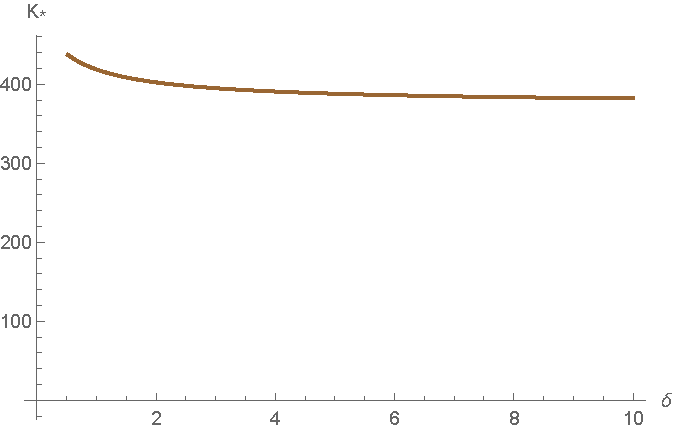
\includegraphics[width=0.32\textwidth]{Prob2_CapOpt/koptx_delta.pdf}}
		\subfigure[$ r \in ( \mu, 1 )$]{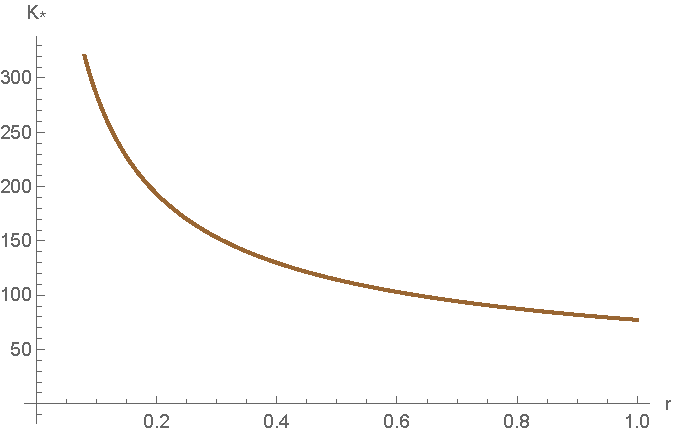
\includegraphics[width=0.32\textwidth]{Prob2_CapOpt/koptx_r.pdf}}
		\subfigure[$ \alpha \in (0,1)$]{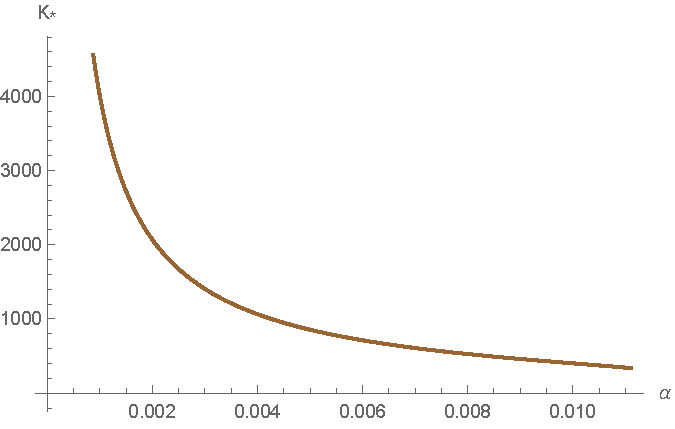
\includegraphics[width=0.32\textwidth]{Prob2_CapOpt/koptx_alpha.pdf}}
	\end{subfigmatrix}
	\caption{Behaviour of the optimal capacity regarding the threshold value $x^*_C$ and decreasing parameters $\delta$ (a), $r$ (b) and $\alpha$ (c).}
	\label{fig:2_k3}
\end{figure}

The most relevant result presented above corresponds to the one shown in Figure \ref{fig:2_k3} (a). The decreasing behaviour of $K^*_C$ is motivated by the fact that a smaller $\delta$ leads to a lower investment cost and therefore the firm is more attracted to invest on a larger capacity.

On Figures \ref{fig:2_k3} (b) and (c) we observe that $K^*_C$ behaves in a similar way as $K^*_C$ analysed in the previous Chapter \ref{chapter:1}, in particular regarding results on Figure \ref{fig:k2}.
%Regarding the sensibility parameter $\delta$, discount rate $r$ and sensibility parameter $\alpha$, we have on Figure \ref{fig:2_k3} that $K^*_C$ decreases with them, as happened in the previous section.



